\chapter{Simulation}

Simulation is an essential step in the control system design. The simulation model should reflect the dynamics property of the controlled target as close as possible. With a simulated model, engineers can first design and test the controller in the virtual environment and then deploy them in the real world. 

The advantage of a simulation-based development is that it will not cause any damage to the original model, which is usually very expensive and hard to build. Second, engineers can obtain the results in the computer faster than in the real world, which means we can get the results of a simulated test way more quickly than a real field test.

This chapter is about the simulation of Piranha. The formulation is based on a 6-DoF non-linear rigid body system. Unlike ground vehicles like rovers and cars, a water surface vehicle like Piranha has much more complicated dynamics because of fluid mechanics.

The most common ways to formulate the EOM of a given system are either through Lagrangian mechanics or Newtonian mechanics. Because the simulation only has one rigid body target, we preferred Newton's Law in this application. However, Newton's Law only holds within the inertial frame. Here, some assumptions are made before the EOM formulation to ensure this condition is met \cite{nahon1996simplified}.

\section{Assumptions}

Before the formulation, we made a few assumptions to rule out some unnecessary factors to consider, such as the Coriolis force and the earth's curvature. The assumptions include:

\begin{enumerate}
    \item The water surface is calm and flat without any curves.
    \item The vehicle is a rigid body with a constant mass. 
    \item The gravitational acceleration is also a constant value.
    \item The simulated world does not rotate.
    \item The fluid has a constant current direction and speed, as well as the wind.
\end{enumerate}

These assumptions make sure that the simulation world frame is inertial. In other words, we can use Newton's Second Law to formulate the equations of motion.

\section{6 DoF State-Space Equations of Motion}

The equation of motion has 6 degrees of freedom. To simplify the formulation, the state vector $\boldsymbol{X}$ is divided into two parts, $\boldsymbol{x}$ and $\boldsymbol{\nu}$.

\begin{equation}
    \boldsymbol{X}=\left[\begin{aligned}
        &\ \boldsymbol{x}\ \\
        &\ \boldsymbol{\nu}\
    \end{aligned}\right]
\end{equation}

We define $\boldsymbol{x}$ as the position vector, $\boldsymbol{\nu}$ as the velocity vector. They are attached to different reference frames, $\boldsymbol{x}$ is attached to the ground NED frame while $\boldsymbol{\nu}$ is linked to Piranha's body frame.

\begin{align}
    \boldsymbol{x} & =[p_n, p_e, p_d, \phi, \theta, \psi]^\top \\
    \boldsymbol{v} & =[u, v, w, p, q, r]^\top
\end{align}

The input vector of the system $\boldsymbol{u}_{\rm PWM}$ consists of the PWM input values for the left and right thrusters. 

We can write the EOM of this system as:

\begin{equation}
    \boldsymbol{M\dot{\nu}}+\boldsymbol{C}(\boldsymbol{x},\boldsymbol{\nu},\boldsymbol{w}_c)+\boldsymbol{D}(\boldsymbol{x}, \boldsymbol{\nu}, \boldsymbol{w}_a)+\boldsymbol{G}=\boldsymbol{\tau}
\end{equation}

$\boldsymbol{M}$ is the mass matrix, $\boldsymbol{C}(\boldsymbol{x},\boldsymbol{\nu},\boldsymbol{w}_c)$ is the fluid dynamical matrix, $\boldsymbol{w}_c$ is the water current vector, $\boldsymbol{D}(\boldsymbol{x}, \boldsymbol{\nu}, \boldsymbol{w}_a)$ is the air dynamical matrix, $\boldsymbol{w}_a$ is the wind speed vector, $\boldsymbol{G}$ is the gravity matrix, $\boldsymbol{\tau}(\boldsymbol{u}_{\rm PWM})$ is the mapped input vector of the system, the transformation will be discussed in after a few sections.

\section{Reference Frames}

In the state-space representation shown above, we represent all components as vectors. However, these vectors in the simulation EOM link to different frames, such as the input vector $\boldsymbol{\tau}(\boldsymbol{u}_{\rm PWM})$ is in the body frame. Meanwhile, the gravitational component $G$ is a constant vector in the ground frame.

To begin with, here list five types of frames in the simulation:

\begin{itemize}
    \item Earth-Centered Inertial (ECI) frame.
    \item Earth-Centered, Earth-Fixed (ECFF) frame.
    \item Ground North, East, Down (NED) frame.
    \item Local North, East, Down frame.
    \item The Body frame.
\end{itemize}

Because the assumptions rule out the world's rotation, the Coriolis effect does not exist in the simulation. Because Piranha only moves on the surface of the earth, we consider the $\boldsymbol{x}$ position vector is in the ground NED frame rather than the ECFF frame and ECI frame.

Since we use Newton's Law for building the simulation EOM, every component inside the equation is relative to the body frame. However, some parts like the wind speed vector and the gravity matrix are initially constant in the local NED frame, so we must transform them into the same frame first.

\subsection{Transform Vectors from Local NED Frame to Body Frame}

With the roll, pitch, yaw angles to be $[\phi, \theta, \psi]$, the transform matrix can be described by:

\begin{equation}
    R_1=\left[\begin{array}{rrr}
        \cos(\psi) & \sin(\psi) & 0  \\
        -\sin(\psi) & \cos(\psi) & 0 \\
        0 & 0 & 1 
    \end{array}\right]
\end{equation}

\begin{equation}
    R_2=\left[\begin{array}{rrr}
        \cos(\theta) & 0 & -\sin(\theta)  \\
        0 & 1 & 0 \\
        \sin(\theta) & 0 & \cos(\theta) 
    \end{array}\right]
\end{equation}

\begin{equation}
    R_3=\left[\begin{array}{rrr}
        1 & 0 & 0  \\
        0 & \cos(\phi) & \sin(\phi) \\
        0 & \sin(\phi) & \cos(\phi) 
    \end{array}\right]
\end{equation}

\begin{equation}
    \boldsymbol{x}_{\rm body}=R_3R_2R_1\boldsymbol{x}_{\rm ground}
\end{equation}

\section{Mass Matrix}

First decompose the velocity vector $\boldsymbol{\nu}$ into linear movement $\boldsymbol{\nu}_l=[u,\ v,\ w]$ and rotation parts $\boldsymbol{\nu}_r=[p,\ q,\ r]$. The mass matrix can also be split into the linear mass matrix $\mathbf{M}_l$ and the inertia matrix $\mathbf{M}_r$.

\begin{equation}
    \mathbf{M}=\left[\begin{array}{cc}
        \mathbf{M}_l & \boldsymbol{0} \\
        \boldsymbol{0} & \mathbf{M}_r
    \end{array}\right]
\end{equation}

Where,

\begin{equation}
    \mathbf{M}_l = m\mathbf{I}\quad \mathbf{M}_r=\left[\begin{array}{ccc}
        I_{xx} & I_{xy} & I_{xz} \\
        I_{yx} & I_{yy} & I_{yz} \\
        I_{zx} & I_{zy} & I_{zz} \\
    \end{array}\right]
\end{equation}

And,

\begin{align}
    \mathbf{F} &=\mathbf{F}_0+\Delta\mathbf{F} \\
    \mathbf{T} &=\mathbf{T}_0+\Delta\mathbf{T}
\end{align}

$\mathbf{F}_0$ and $\mathbf{T}$ is the theoretical force and torque. The $\Delta$ denotes the perturbation in the real-world model. In this section, we ignore this perturbation.

With Newton's Law,

\begin{equation}
    \mathbf{F}=\left[\begin{array}{ccc}
        m\dot{u} & \cdots & 0 \\
        \vdots & m\dot{v} & \vdots\\
        0 & \cdots & m\dot{w}
    \end{array}\right]\quad \mathbf{T}=\left[\begin{array}{ccc}
        I_{xx} & I_{xy} & I_{xz} \\
        I_{yx} & I_{yy} & I_{yz} \\
        I_{zx} & I_{zy} & I_{zz}
    \end{array}\right]\left[\begin{array}{c}
        \dot{p} \\
        \dot{q} \\
        \dot{r}
    \end{array}\right]
\end{equation}

\begin{equation}
    \mathbf{M}\dot{\mathbf{\nu}}=\left[\begin{array}{cc}
        \mathbf{F} & \boldsymbol{0}  \\
        \boldsymbol{0} & \mathbf{T}
    \end{array}\right]
\end{equation}

In the simulation, these values are obtained from SOLIDWORKS Mass Properties, shown in Figure \ref{fig:04mass}:

\begin{figure}[ht]
    \centering
    \includegraphics[width=.5\textwidth]{images/04solidworks.png}
    \caption{The mass matrix values of Piranha generated in the SOLIDWORKS Mass Properties menu.}
    \label{fig:04mass}
\end{figure}

\section{Fluid Dynamical Model}

The fluid dynamical model includes two parts, hydrostatic and hydrodynamic parts.

\subsection{Hydrostatic analysis}

In the hydrostatic part, the goal of the simulator is to estimate the whole buoyant force applied to Piranha and the buoyancy center, given the position of the boat. In Figure \ref{fig:04smodel}, we can see that the buoyancy estimation includes the center of buoyancy estimation and the upward force estimation. According to Archimedes' principle, we can calculate the upward buoyant force through the volume of the displaced water. 


\begin{figure}
    \centering
    \includegraphics[width=.8\textwidth]{images/04hydrostatic.pdf}
    \caption{Hydrostatic model of Piranha.}
    \label{fig:04smodel}
\end{figure}

We can get estimations with pure mathematical calculation. For simplicity, here we do the math in the body frame. The first step is to transform the water level back to the Piranha's body frame, shown in the following equation.

\begin{equation}
    F_{wg}(x,y)=0 \longrightarrow F_{wb},\quad F_{wg}, \ F_{wb} \in R^2 
\end{equation}

We can consider the water level surface as a plane under the assumptions. So the equation of a plane in 3D space is:

\begin{equation}
    ax+by+cz=d
\end{equation}

The normal vector can be represented as $\boldsymbol{n_1}=[a, b, c]^\top$. We can determine the water surface in the body frame by solving this equation:

\begin{equation}
        R_v^b\boldsymbol{n_1} \cdot \boldsymbol{x}^\top_{(x=0,y=0)} = p_d
\end{equation}

There are three cases in calculating integral:

\begin{enumerate}
    \item The water level surface only intersects the lower half part of the float.
    \item The water level surface only intersects the upper half part of the float.
    \item The water level surface intersects both the upper and lower halves of the float.
\end{enumerate}

For all three cases, the integral can be represented as the following equation, denote $F_s$ to be the separate plane:

\begin{equation}
    V=\iint_{A_{xy}} \left[\min(\max(F_w-F_s,0),F_u-F_s) + \min(\max(F_w-F_l,0),F_s-F_l)\right]
\end{equation}

Because it is not a differentiable function due to $min$ and $max$ operators, but it can be solved using modern numerical methods. The formulation is not exclusive. These variables inside the integrated function can be $(x,z)$ instead of $(x,y)$. However, the function is always not differentiable. 

The buoyancy center is the mass center of the displaced water, thus can be calculated by the center of mass formula:

\begin{align}
    & M_{yz} =\iiint x\rho(x,y,z)\ {\rm d}V \\
    & M_{xz} =\iiint y\rho(x,y,z)\ {\rm d}V \\
    & M_{xy} =\iiint z\rho(x,y,z)\ {\rm d}V \\
    & \overline{x} =\frac{M_{yz}}{m},\ \overline{y} =\frac{M_{xz}}{m},\ \overline{z} =\frac{M_{xy}}{m}
\end{align}

\subsection{Hydrodynamic analysis}

The hydrodynamic analysis calculates the parasitic forces in the simulation. This process in real-life applications is usually handled by using modern CFD simulators to solve the Navier-Stokes equations. 

Although the CFD simulation precision depends on the fineness of the mesh, limited by today's computer technology, the CFD simulation is not real-time. Usually, it takes a long time, ranging from a few minutes to hours, to calculate for a set of given parameters. However, the CFD simulation needs to run from tens to thousands of times per second in the simulation scenarios, depending on the time step. As a result, the time cost for calculating hydrodynamics using common CFD software is unacceptable in the simulation.

The following section introduces an algorithm, which is used in Piranha's simulation code. This algorithm takes a triangle mesh as the input model and does the hydrostatic and hydrodynamic estimation at the cell level first. After that, it sums up all results and produces a general estimate of the buoyancy and drag on the whole body of the boat.

\section{Numerical Calculation}

This section covers the numerical methods used in Piranha's simulation program. We cannot calculate the theoretical equation efficiently in the computer. As a result, a simplified mesh model of Piranha is used to accelerate the calculation.

\subsection{Mesh Simplification}

The first step is to simplify the mesh and reduce the number of triangles to reduce the calculation time cost. The aim is to use the fewest triangles but maintain the shape of the original model.

We represent Piranha's simulation model with two cylinders and two cones, shown in Figure \ref{fig:04mesh}. 

\begin{figure}[H]
     \centering
     \hspace{1cm}
     \begin{subfigure}[b]{0.4\textwidth}
         \centering
         \includegraphics[width=\textwidth]{images/04orca_pontoon.pdf}
     \end{subfigure}
     \hfill
     \begin{subfigure}[b]{0.4\textwidth}
         \centering
         \includegraphics[width=\textwidth]{images/04mesh_orca.pdf}
     \end{subfigure}
     \caption{On the left is the original mesh generated by SOLIDWORKS, on the right is the simplified mesh model.}
     \label{fig:04mesh}
     \hspace{1cm}
\end{figure}

\subsubsection{Buoyancy Estimate}

The key to estimating buoyancy is to calculate the submerged volume. For a single triangle in the mesh, we can calculate its volume by the surface integral over the projected area, shown in the following equations.

\begin{equation}
    \boldsymbol{V} = \int_S F(x,y)\ {\rm d}x{\rm d}y
\end{equation}
   
\begin{equation}
    F(x,y)= \left\{\begin{aligned}
        f(x,y) &, f(x,y)>0 \\
        0 &, f(x,y)\leq 0
    \end{aligned}\right.
\end{equation} 

Given the triangle plane function $z=f(x,y)$.

If we ignore every triangle that is not fully submerged, there is also another way to calculate the volume under a triangle without using integration.

If we have a 3D triangle defined by $(x_1,y_1,z_1)$, $(x_2,y_2,z_2)$, $(x_3,y_3,z_3)$. Assume they are arranged in the order that $z_1<z_2<z_3$.

Assume there is a horizontal plane $P$, in other words, a plane that is parallel to $XY$ plane crossing the middle point $(x_2,y_2,z_3)$, $P$ divides the 3D triangle into upper and lower parts like Figure \ref{fig:04triangle-volume}.

\begin{figure}[ht]
    \centering
    \includegraphics[width=.8\textwidth]{images/04triangle-volume.pdf}
    \caption{$A_1$ and $A_2$ are the projected area of the upper part and the lower part on the plane $P$.}
    \label{fig:04triangle-volume}
\end{figure}

We can calculate the volume of the 3D triangle given above as the volume of the triangular prism made by $P$, plus the upper triangular cone, minus the lower triangular cone, equals to:

\begin{equation}
    V=(A_1+A_2)z_2+\frac{1}{3}A_1(z_3-z_2)-\frac{1}{3}A_2(z_2-z_1)
\end{equation}

The projected area $A_1$ and $A_2$ can be calculated by:

\begin{align}
    A_1  & =  \frac{1}{2}[(x_4y_2-x_2y_4)+(x_3y_4-x_4y_3)+(x_2y_3-x_3y_2)] \\
    A_2  & =  \frac{1}{2}[(x_1y_2-x_2y_1)+(x_4y_1-x_1y_4)+(x_2y_4-x_4y_2)]
\end{align}

Where $(x_4,y_4,z_4)$ is the intersection point between $(x_3,y_3,z_3)$ and $(x_1,y_1,z_1)$. Apparently because $(x_4, y_4, z_4)$ is on $P$, $z_4=z_2$. $x_4$ and $y_4$ are given by:

\begin{align}
    x_4 &= x_1 + ((z_2-z_1)/(z_3-z_1)) (x_3-x_1) \\
    y_4 &= y_1 + ((z_2-z_1)/(z_3-z_1)) (y_3-y_1)
\end{align}

Substitute back and simplify the equation. In the end, the volume under a 3D triangle can be calculated by:

\begin{equation}
    V_{tri}  =  \frac{1}{6}(z_1+z_2+z_3)(A_1+A_2)=\frac{1}{6}(z_1+z_2+z_3)A_{proj}
\end{equation}

The volume equation can be interpreted as the "average height" times the projected area times $1/2$.

We can calculate the projected area through the cross product:

\begin{equation}
    A_{proj}=\frac{1}{2}|\boldsymbol{u}\times\boldsymbol{v}|
\end{equation}

There is no need for the computational heavy integration step when calculating the volume with this volume formula. However, we can only use it when the triangle is fully submerged.

However, if a triangle is not fully submerged, it is either partially submerged or not submerged at all. For the latter case, we can ignore the triangle. For the partially submerged case, there are two chances:

\begin{enumerate}
    \item Only one vertex is in the water.
    \item Two vertices are in the water.
\end{enumerate}

The simulator takes extra steps for these two cases, shown in Figure \ref{fig:04two-cases}. The key is to find the two intersection points and calculate the cone volume.


\begin{align}
    \text{For case 1:} & \quad V=V_{cone} \\
    \text{For case 2:} & \quad V=V_{tri}+V_{cone}
\end{align}

\begin{figure}[ht]
    \centering
    \includegraphics[width=.8\textwidth]{images/04two-cases.pdf}
    \caption{Two partially submerged cases.}
    \label{fig:04two-cases}
\end{figure}

Given the volume formula, it is easy to calculate the underwater volume for one triangular cell. The next step is to repeat this step for each triangle and sum up the results.

The face direction determines the volume should be taken from the sum, or added to the result, shown in Figure \ref{fig:04face-direction}. 

\begin{figure}[ht]
    \centering
    \includegraphics[width=.6\textwidth]{images/04face-direction.pdf}
    \caption{The offset water volume is between the two triangles. The face directions for the two triangles are different.}
    \label{fig:04face-direction}
\end{figure}

During the calculation, the program determines the face direction by the normal vector of the triangle. Due to this fact, the simulator saves the normal vectors and the triangle mesh for further calculation. These normal vectors, if visualized, can be seen in Figure \ref{fig:04normal-vector}:

\begin{figure}[H]
    \centering
    \includegraphics[width=.6\textwidth]{images/04normal-vector.pdf}
    \caption{In the mesh model, the area of a triangular face equals the length of its normal vector.}
    \label{fig:04normal-vector}
\end{figure}

Figure \ref{fig:04hydrostatic-flowchart} briefly illustrates the flowchart of the buoyancy estimate algorithm. However, in practice, the simulator does not follow this chart strictly. In the real world, the simulator combines the hydrostatic estimator and hydrodynamic estimator so that the face classification process only needs to run once for each face. The classification result is shared between both estimators for performance optimization.  

\begin{figure}[H]
    \centering
    \includegraphics[width=\textwidth]{images/04hydrostatics_flowchart.pdf}
    \caption{Piranha's hydrostatic estimator flowchart.}
    \label{fig:04hydrostatic-flowchart}
\end{figure}

\subsubsection{Drag \& Skin Friction Estimate}

For simplicity, we only consider drag and skin friction in the simulation's hydrodynamics. The other factor like water waves and twirls are not considered here \cite{tian2015dynamic}. We can calculate these two forces through:

\begin{equation}
\begin{split}
    F_d &= \int C_{i0}+ C_{i1} \rho v_1 + C_{i2} \rho v_1^2  {\rm d} A \\
    F_f &= \int C_{f0}+ C_{f1} \rho v_2 C_{f2} \rho v_2^2 {\rm d} A
\end{split}
\end{equation}

However, unlike most common simulators, which only use a rough frontal area value in the formula, Piranha's simulator uses a more precise algorithm to calculate the frontal area.

The drag and skin friction are calculated independently for each triangular cell. The simulator sums up all the result values and synthesizes a general force and general torque to represent the hydrodynamic component, shown in Figure \ref{fig:04orca_surf}.

\begin{figure}
    \centering
    \includegraphics[width=.8\textwidth]{images/04orca_surf.pdf}
    \caption{Cell level dynamics, drag and skin friction.}
    \label{fig:04orca_surf}
\end{figure}

The hydrodynamics estimator flowchart can be found in Figure \ref{fig:04hydrodynamic-flowchart}.

\begin{figure}
    \centering
    \includegraphics[width=\textwidth]{images/04hydrodynamics_flowchart.pdf}
    \caption{Piranha's hydrodynamic estimator flowchart.}
    \label{fig:04hydrodynamic-flowchart}
\end{figure}

The flowchart shows that each face is classified into different types according to the above discussion first. And for simplicity, the simulator ignores the skin friction component for the area in the air.

\subsubsection{Wind and Current Vectors}

Wind and water current have a significant effect on the simulation. Thus, the simulator cannot ignore them blindly. However, compared with hydrodynamics, the aerodynamics of Piranha is of less importance.

In the simulation, these factors are considered in the hydrodynamics estimation part, as shown in Figure \ref{fig:04hydrodynamic-flowchart}. While calculating the drag and friction for a face, the simulator first calculates a relative speed for the wind frame and water current frame, then proceeds to the movement decoupling step and applies drag and skin friction coefficients correspondingly.

\section{Input Mapping}

The simulation input is the PWM control signal widths of the two thrusters, which are controllable by the embedded controller. However, the PWM pulse widths need to be transformed into propulsion forces first.

According to the BlueRobotics lab tests results attached to this report in the Appendix section \ref{app:t200}, the propulsion force depends on two factors, the voltage, and the PWM pulse width. We can see the data in Figure \ref{fig:04thruster-curve}.

\begin{figure}[H]
    \centering
    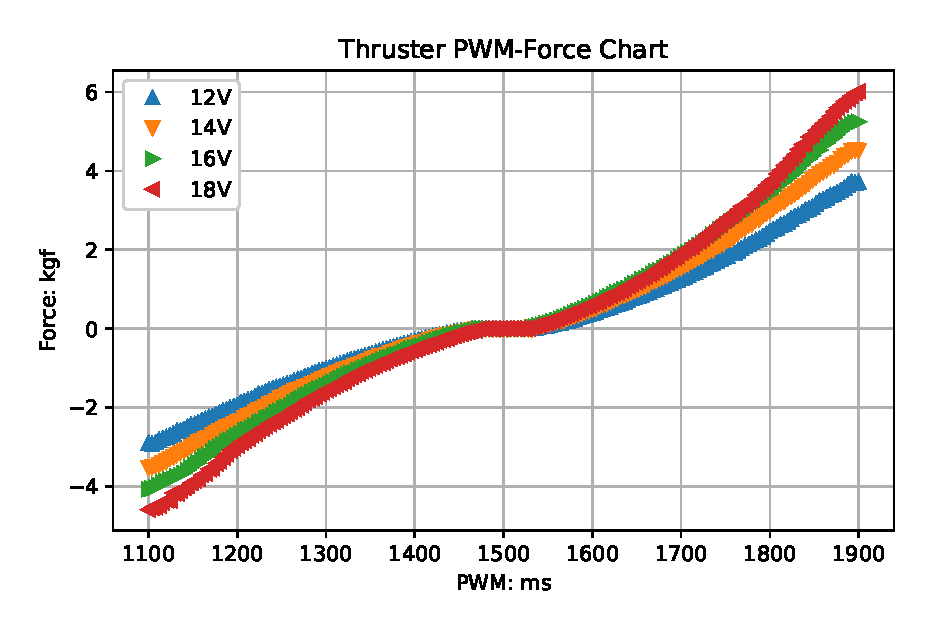
\includegraphics[width=\textwidth]{images/04thruster-curve.eps}
    \caption{BlueRobotics T200 Thruster input-output curve according to the lab test.}
    \label{fig:04thruster-curve}
\end{figure}

The input mapping part in the simulator transforms the input PWM values to the propulsion forces generated by the two thrusters. It works using the nearest point algorithm. At first, it determines which curve to look for the nearest point, then finds the dot with the closest PWM value.

\begin{equation}
    \boldsymbol{u}_{\rm f}=\boldsymbol{F}_{\Delta}(\boldsymbol{u}_{\rm PWM})
\end{equation}

The next step is to obtain the torque. According to the geometry definition of the thrusters, the torque can be calculated through the cross-product of the position vector and the propulsion force. 

\begin{equation}
    \boldsymbol{u}_{\rm q}=\boldsymbol{v_t}\times \boldsymbol{u}_{\rm f}
\end{equation}

And at last,

\begin{equation}
    \boldsymbol{\tau}=\left[\begin{array}{c}
        \boldsymbol{u}_{\rm f}  \\
        \boldsymbol{u}_{\rm q}
    \end{array}\right]
\end{equation}

Which is the right hand side of the EOM \cite{sonnenburg2013modeling}.

\section{Simulation Results}

After building the simulator, we tuned all parameters based on the position and speed data collected during the real-world tests to ensure the simulation was valid. Some parameters are fixed by the mechanical design, such as the gravity center and the mass matrix, so they are determined beforehand. 

Other parameters, including the water drag and skin friction coefficients and air drag coefficient (we set the simulator to have a zero skin coefficient for air skin friction), are changeable.

Readers can find three test results in the following few sections.

\subsection{Drop Test}

Drop test is the most straightforward test. In this test, we put Piranha at a certain height above the water at the beginning. When time starts, Piranha starts free-falling until it reaches a stable position where the buoyancy and weight are equal.

Because the input vector is zero all the time, this test can be used to verify the hydrostatic estimator and hydrodynamics estimator work properly. The results are shown in Figure \ref{fig:04drop-test-xyz}, \ref{fig:04drop-test-ptp}, \ref{fig:04drop-test-uvw}, \ref{fig:04drop-test-pqr}.

\begin{figure}[H]
    \centering
    \includegraphics[width=.8\textwidth]{images/04drop-test-xyz.eps}
    \caption{Simulation: Drop test result - Positions $x, y,z$}
    \label{fig:04drop-test-xyz}
\end{figure}

\begin{figure}[H]
    \centering
    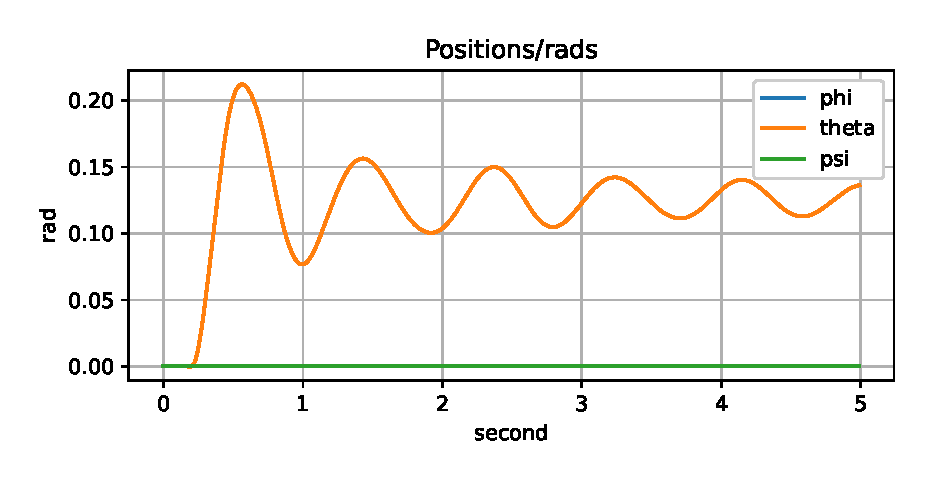
\includegraphics[width=.8\textwidth]{images/04drop-test-ptp.eps}
    \caption{Simulation: Drop test result - Attitude $\phi, \theta, \psi$}
    \label{fig:04drop-test-ptp}
\end{figure}

\begin{figure}[H]
    \centering
    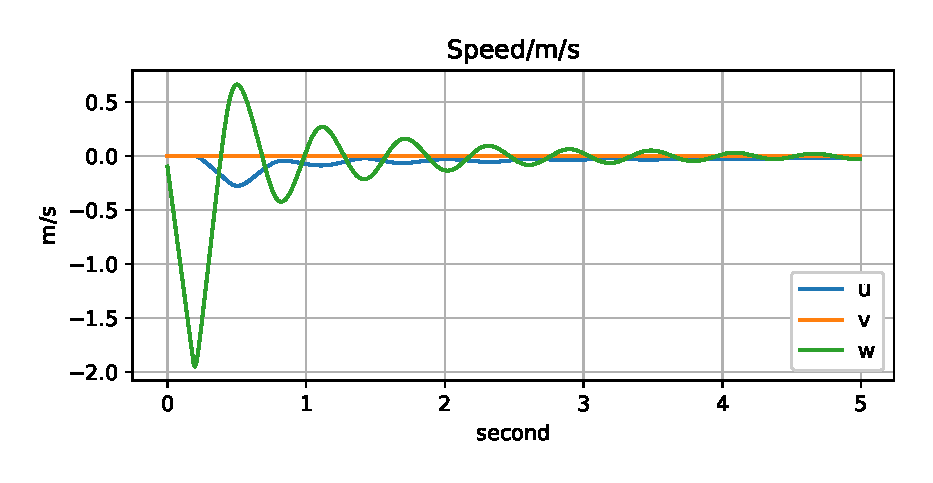
\includegraphics[width=.8\textwidth]{images/04drop-test-uvw.eps}
    \caption{Simulation: Drop test result - Linear Speed $u, v, w$}
    \label{fig:04drop-test-uvw}
\end{figure}

\begin{figure}[H]
    \centering
    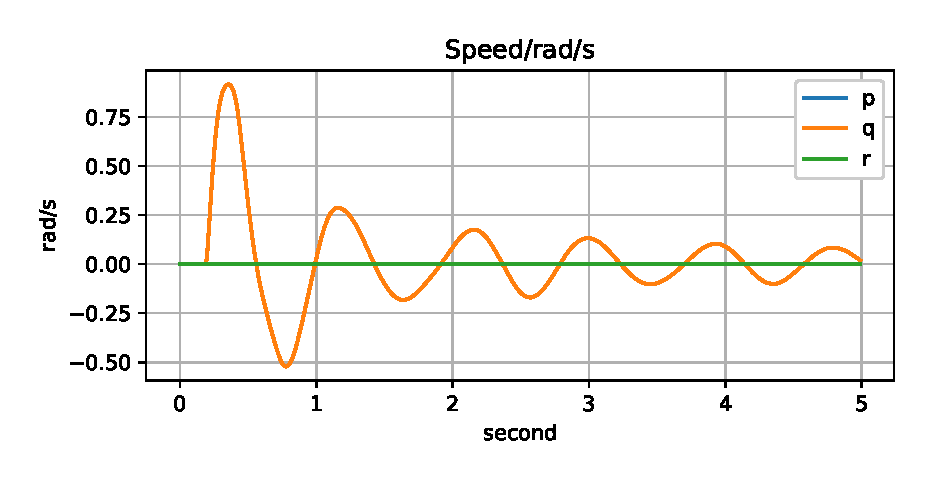
\includegraphics[width=.8\textwidth]{images/04drop-test-pqr.eps}
    \caption{Simulation: Drop test result - Angular Speed $p, q, r$}
    \label{fig:04drop-test-pqr}
\end{figure}

\subsection{Linear Driving Test}

In the Linear driving test, Piranha starts at a stable state, with a zero speed. When the test starts, the left and right thrusters move forward at maximum input values. The test results are shown in Figure \ref{fig:04linear-test-xyz}, \ref{fig:04linear-test-ptp}, \ref{fig:04linear-test-uvw}, \ref{fig:04linear-test-pqr}.

\begin{figure}[H]
    \centering
    \includegraphics[width=.8\textwidth]{images/04linear-test-xyz.eps}
    \caption{Simulation: Linear driving test result - Positions $x, y,z$}
    \label{fig:04linear-test-xyz}
\end{figure}

\begin{figure}[H]
    \centering
    \includegraphics[width=.8\textwidth]{images/04linear-test-ptp.eps}
    \caption{Simulation: Linear driving test result - Attitude $\phi, \theta, \psi$}
    \label{fig:04linear-test-ptp}
\end{figure}

\begin{figure}[H]
    \centering
    \includegraphics[width=.8\textwidth]{images/04linear-test-uvw.eps}
    \caption{Simulation: Linear driving test result - Linear Speed $u, v, w$}
    \label{fig:04linear-test-uvw}
\end{figure}

\begin{figure}[H]
    \centering
    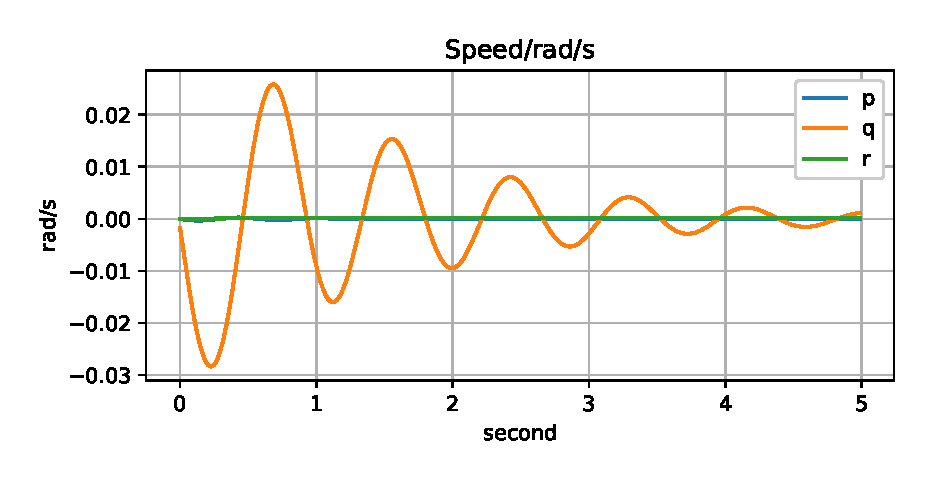
\includegraphics[width=.8\textwidth]{images/04linear-test-pqr.eps}
    \caption{Simulation: Linear driving test result - Angular Speed $p, q, r$}
    \label{fig:04linear-test-pqr}
\end{figure}

\subsection{Steering Test}

Steering test starts Piranha at the equilibrium point, then the left thruster is given a maximum forward input value, the right thruster is given a maximum backward input value. As a result, the Piranha starts turning. The simulation results can be found in Figure \ref{fig:04steer-test-xyz}, \ref{fig:04steer-test-ptp}, \ref{fig:04steer-test-uvw}, \ref{fig:04steer-test-pqr}.

\begin{figure}[H]
    \centering
    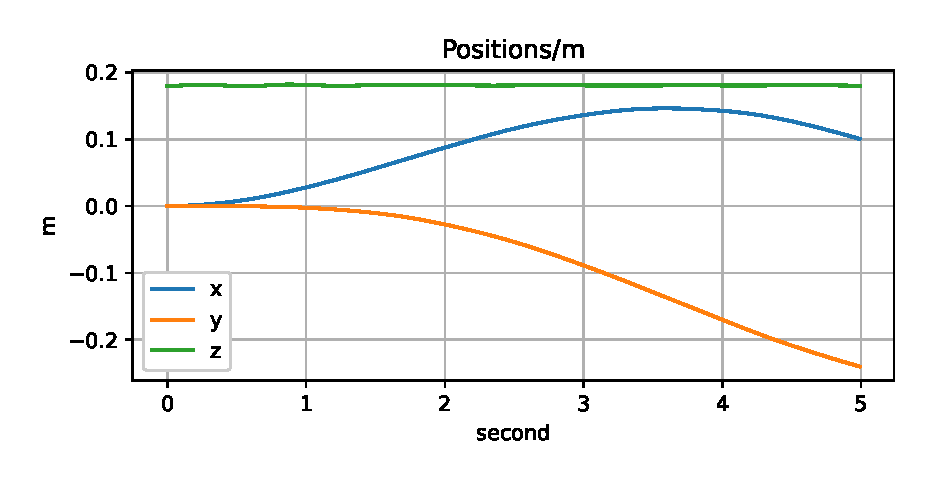
\includegraphics[width=.8\textwidth]{images/04steer-test-xyz.eps}
    \caption{Simulation: Steering test result - Positions $x, y,z$}
    \label{fig:04steer-test-xyz}
\end{figure}

\begin{figure}[H]
    \centering
    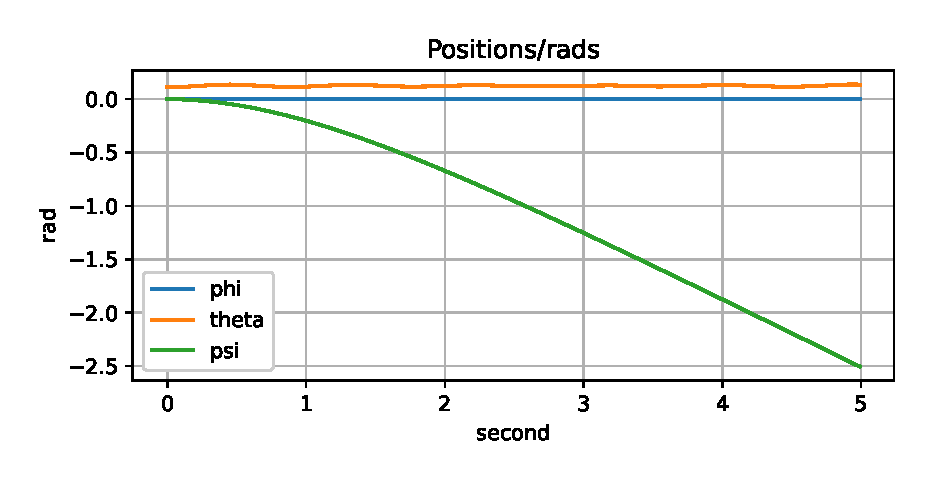
\includegraphics[width=.8\textwidth]{images/04steer-test-ptp.eps}
    \caption{Simulation: Steering test result - Attitude $\phi, \theta, \psi$}
    \label{fig:04steer-test-ptp}
\end{figure}

\begin{figure}[H]
    \centering
    \includegraphics[width=.8\textwidth]{images/04steer-test-uvw.eps}
    \caption{Simulation: Steering test result - Linear Speed $u, v, w$}
    \label{fig:04steer-test-uvw}
\end{figure}

\begin{figure}[H]
    \centering
    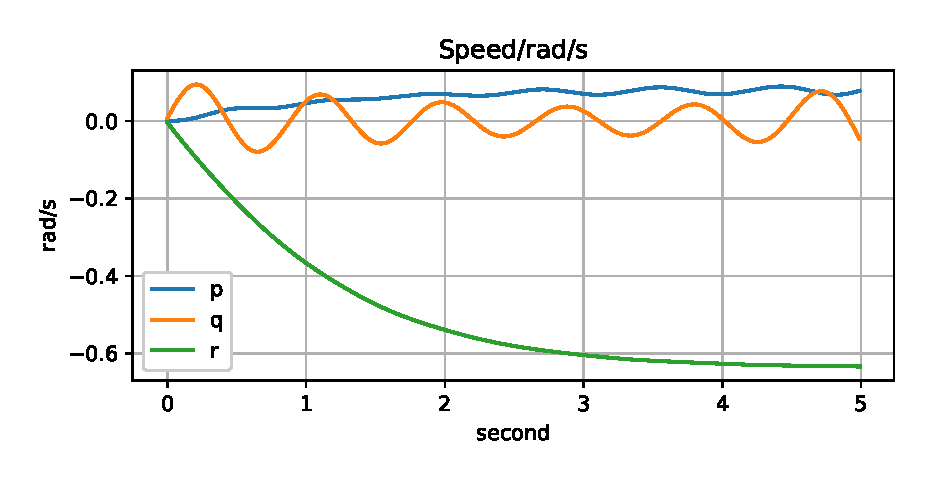
\includegraphics[width=.8\textwidth]{images/04steer-test-pqr.eps}
    \caption{Simulation: Steering test result - Angular Speed $p, q, r$}
    \label{fig:04steer-test-pqr}
\end{figure}